\chapter{Requirements Analysis and Specification}
\label{chap:requirements}

\section*{Introduction}

This chapter identifies the three system actors, formalises the
functional and non-functional requirements of the platform, and
illustrates them with UML use-case and class diagrams. It then presents
the Scrum management of the project --- the team, the product backlog
and the sprint planning --- followed by the schedule and the
architecture and technical choices that underpin the realisation.

\section{Requirements Specification}

\subsection{Identification of Actors}

The platform recognises three actor categories. They are distinct
\textit{roles} stored on the \texttt{User} table rather than distinct
user records: a single account can be promoted from \textit{customer}
to \textit{seller} once a seller application is approved, and an
administrator account is created automatically on first boot.

\begin{itemize}[leftmargin=*,itemsep=4pt]
  \item \textbf{Customer.} The default role assigned upon registration.
        A Customer can browse the catalogue, search products, view
        individual stores, manage a cart, place an order across multiple
        sellers in a single checkout, and review their order history.
        Any Customer can submit a seller application and, once approved,
        gain the Seller role on the same account. Anonymous visitors
        share the read-only abilities of the Customer but cannot
        maintain a cart or place an order.
  \item \textbf{Seller.} A Customer whose seller application has been
        approved by an administrator. A Seller can create and edit one
        store under the free tier (or several under the premium tier),
        populate it with products, upload product images, attach product
        tags, choose a visual template, and consult the orders specific
        to their store. Sellers cannot review or moderate the work of
        other sellers.
  \item \textbf{Administrator.} Created automatically by the backend at
        first boot and not exposed through registration. The
        Administrator reviews seller applications, browses every store
        and product, suspends or deletes stores (with cascading
        deletion), overrides automated AI verification decisions,
        curates featured content, manages categories, and consults the
        platform through a database-aware AI chat assistant.
\end{itemize}

\subsection{Functional Requirements}

The functional requirements are grouped into seven domains. Each domain
corresponds to a backend NestJS module and to a matching set of pages on
the React frontend.

\paragraph{User Registration and Authentication.}
\begin{enumerate}[label=\textbf{FR-A\arabic*.},leftmargin=*,itemsep=1pt]
  \item The system shall allow a visitor to create an account with an
        email address and password.
  \item The system shall send a verification email containing a one-time
        link upon successful registration.
  \item The system shall prevent unverified accounts from creating a
        store or placing an order.
  \item The system shall authenticate returning users via Better-Auth
        sessions and issue an HTTP-only cookie.
  \item The system shall allow the user to log out and invalidate the
        corresponding session.
  \item The system shall enforce role-based access control on every
        non-public route through guards and a \texttt{@Roles()}
        decorator.
\end{enumerate}

\paragraph{Store Management.}
\begin{enumerate}[label=\textbf{FR-S\arabic*.},leftmargin=*,itemsep=1pt]
  \item A Seller shall create a store with a name, description, logo and
        template, and edit it at any time.
  \item A free-tier Seller shall be limited to a single store; a
        premium-tier Seller shall operate multiple stores.
  \item Each store shall expose a public storefront URL identified by a
        human-readable slug derived from its name, with uniqueness
        enforced and the slug regenerated when the name changes.
  \item The Seller shall customise the storefront across seven
        independent sections (theme, announcement bar, banner, header,
        product grid, sidebar, footer) through a WYSIWYG visual editor,
        with undo/redo and selectable presets.
  \item Customisation features shall be tiered: free accounts use a
        curated subset, while premium accounts unlock the full set; on
        premium expiry, existing customisation is preserved but no
        longer editable.
  \item A Seller shall activate a store-wide percentage sale that
        propagates a discounted price and a sale badge across product
        cards, the store card and search results, and applies at
        checkout.
  \item A Seller shall trigger an AI-assisted storefront redesign by
        submitting a natural-language prompt, which generates a complete
        customisation applied live to the editor for review.
\end{enumerate}

\paragraph{Product Management.}
\begin{enumerate}[label=\textbf{FR-P\arabic*.},leftmargin=*,itemsep=1pt]
  \item A Seller shall create, edit and delete products in their own
        store(s).
  \item Each product shall accept one or more images of validated type
        and size, and an arbitrary number of tags used by the
        recommendation engine.
  \item Each product shall carry an \texttt{aiReviewed} flag set by the
        verification pipeline and an \texttt{adminReviewed} flag set on
        manual override.
  \item Products shall be browsable by category and sub-category.
\end{enumerate}

\paragraph{Order System.}
\begin{enumerate}[label=\textbf{FR-O\arabic*.},leftmargin=*,itemsep=1pt]
  \item A Customer shall add and remove items in a client-side cart.
  \item Checkout shall create a single order even when the cart spans
        multiple stores, with one order item per product line, and
        trigger a confirmation email.
  \item Each Customer shall consult their order history and each Seller
        the orders that include at least one of their products.
\end{enumerate}

\paragraph{Administration.}
\begin{enumerate}[label=\textbf{FR-D\arabic*.},leftmargin=*,itemsep=1pt]
  \item The Administrator shall access a dashboard listing pending
        seller applications, recent activity and platform statistics.
  \item The Administrator shall approve or reject seller applications,
        granting the Seller role on approval.
  \item The Administrator shall suspend, reactivate or delete any store,
        with cascading deletion of its products and orders, and override
        any AI verdict.
\end{enumerate}

\paragraph{AI Verification.}
\begin{enumerate}[label=\textbf{FR-V\arabic*.},leftmargin=*,itemsep=1pt]
  \item Once its images are uploaded, every store and product shall be
        submitted to an n8n verification workflow that screens each
        image together with the listing text using a hosted multimodal
        large-language model.
  \item The workflow shall return a decision (\textit{approve} or
        \textit{flag}) with a textual rationale, written back to the
        entity through a callback endpoint.
  \item Flagged entities shall appear in the moderation queue for
        administrative review.
\end{enumerate}

\paragraph{Featured Content Curation.}
\begin{enumerate}[label=\textbf{FR-C\arabic*.},leftmargin=*,itemsep=1pt]
  \item The Administrator shall mark any store or product as
        \textit{featured}, promoting it on the landing page.
  \item In the absence of featured products for a tag, the
        recommendation engine shall fall back to top-selling products of
        that tag.
\end{enumerate}

\subsection{Non-Functional Requirements}

Beyond pure functionality, the deliverable must exhibit the qualities
summarised in Table~\ref{tab:nfr}, prioritised with the professional
supervisor during the requirements review.

\begin{table}[H]
  \centering
  \caption{Non-functional requirements}
  \label{tab:nfr}
  \begin{tabularx}{\textwidth}{|l|X|}
    \hline
    \rowcolor{tableHeader}
    \textcolor{white}{\textbf{Criterion}} & \textcolor{white}{\textbf{Description}} \\
    \hline
    Performance      & Catalogue and store pages render in under one second on a 10\,Mbit/s connection; typical API endpoints respond in under 300\,ms. \\ \hline
    Security         & Passwords hashed by Better-Auth; sessions in HTTP-only, \texttt{SameSite=Lax} cookies; HTTP security headers via Helmet; uploads validated by type and size; every protected route gated by an auth guard and the \texttt{@Roles()} decorator, with object-level ownership enforced in the service layer. Required secrets are validated at start-up. \\ \hline
    Scalability      & The backend is stateless and horizontally scalable behind a reverse proxy; uploads live on a volume that can migrate to object storage with no code change. \\ \hline
    Availability     & The production stack runs under Docker Compose with restart policies; deployment is zero-downtime through rolling container replacement. \\ \hline
    Usability        & The frontend follows accessible component patterns, is fully responsive, and uses slug-based, human-readable URLs. \\ \hline
    Maintainability  & The codebase is split into bounded NestJS modules, the schema is versioned through Prisma migrations, and the infrastructure is reproducible through Terraform. \\ \hline
    Observability    & Application logs are emitted to \texttt{stdout} and aggregated by Docker; the chat assistant offers a queryable view of the database for diagnostics. \\ \hline
  \end{tabularx}
\end{table}

\section{Global Use-Case Diagram}

Figure~\ref{fig:uc-global} groups the principal use cases of the
platform around its three actors. Two dotted dependencies illustrate the
cross-actor flows on which the rest of the analysis relies: a seller
application \emph{triggers} an administrative review, and product
creation is automatically \emph{verified by AI}.

\begin{figure}[H]
  \centering
  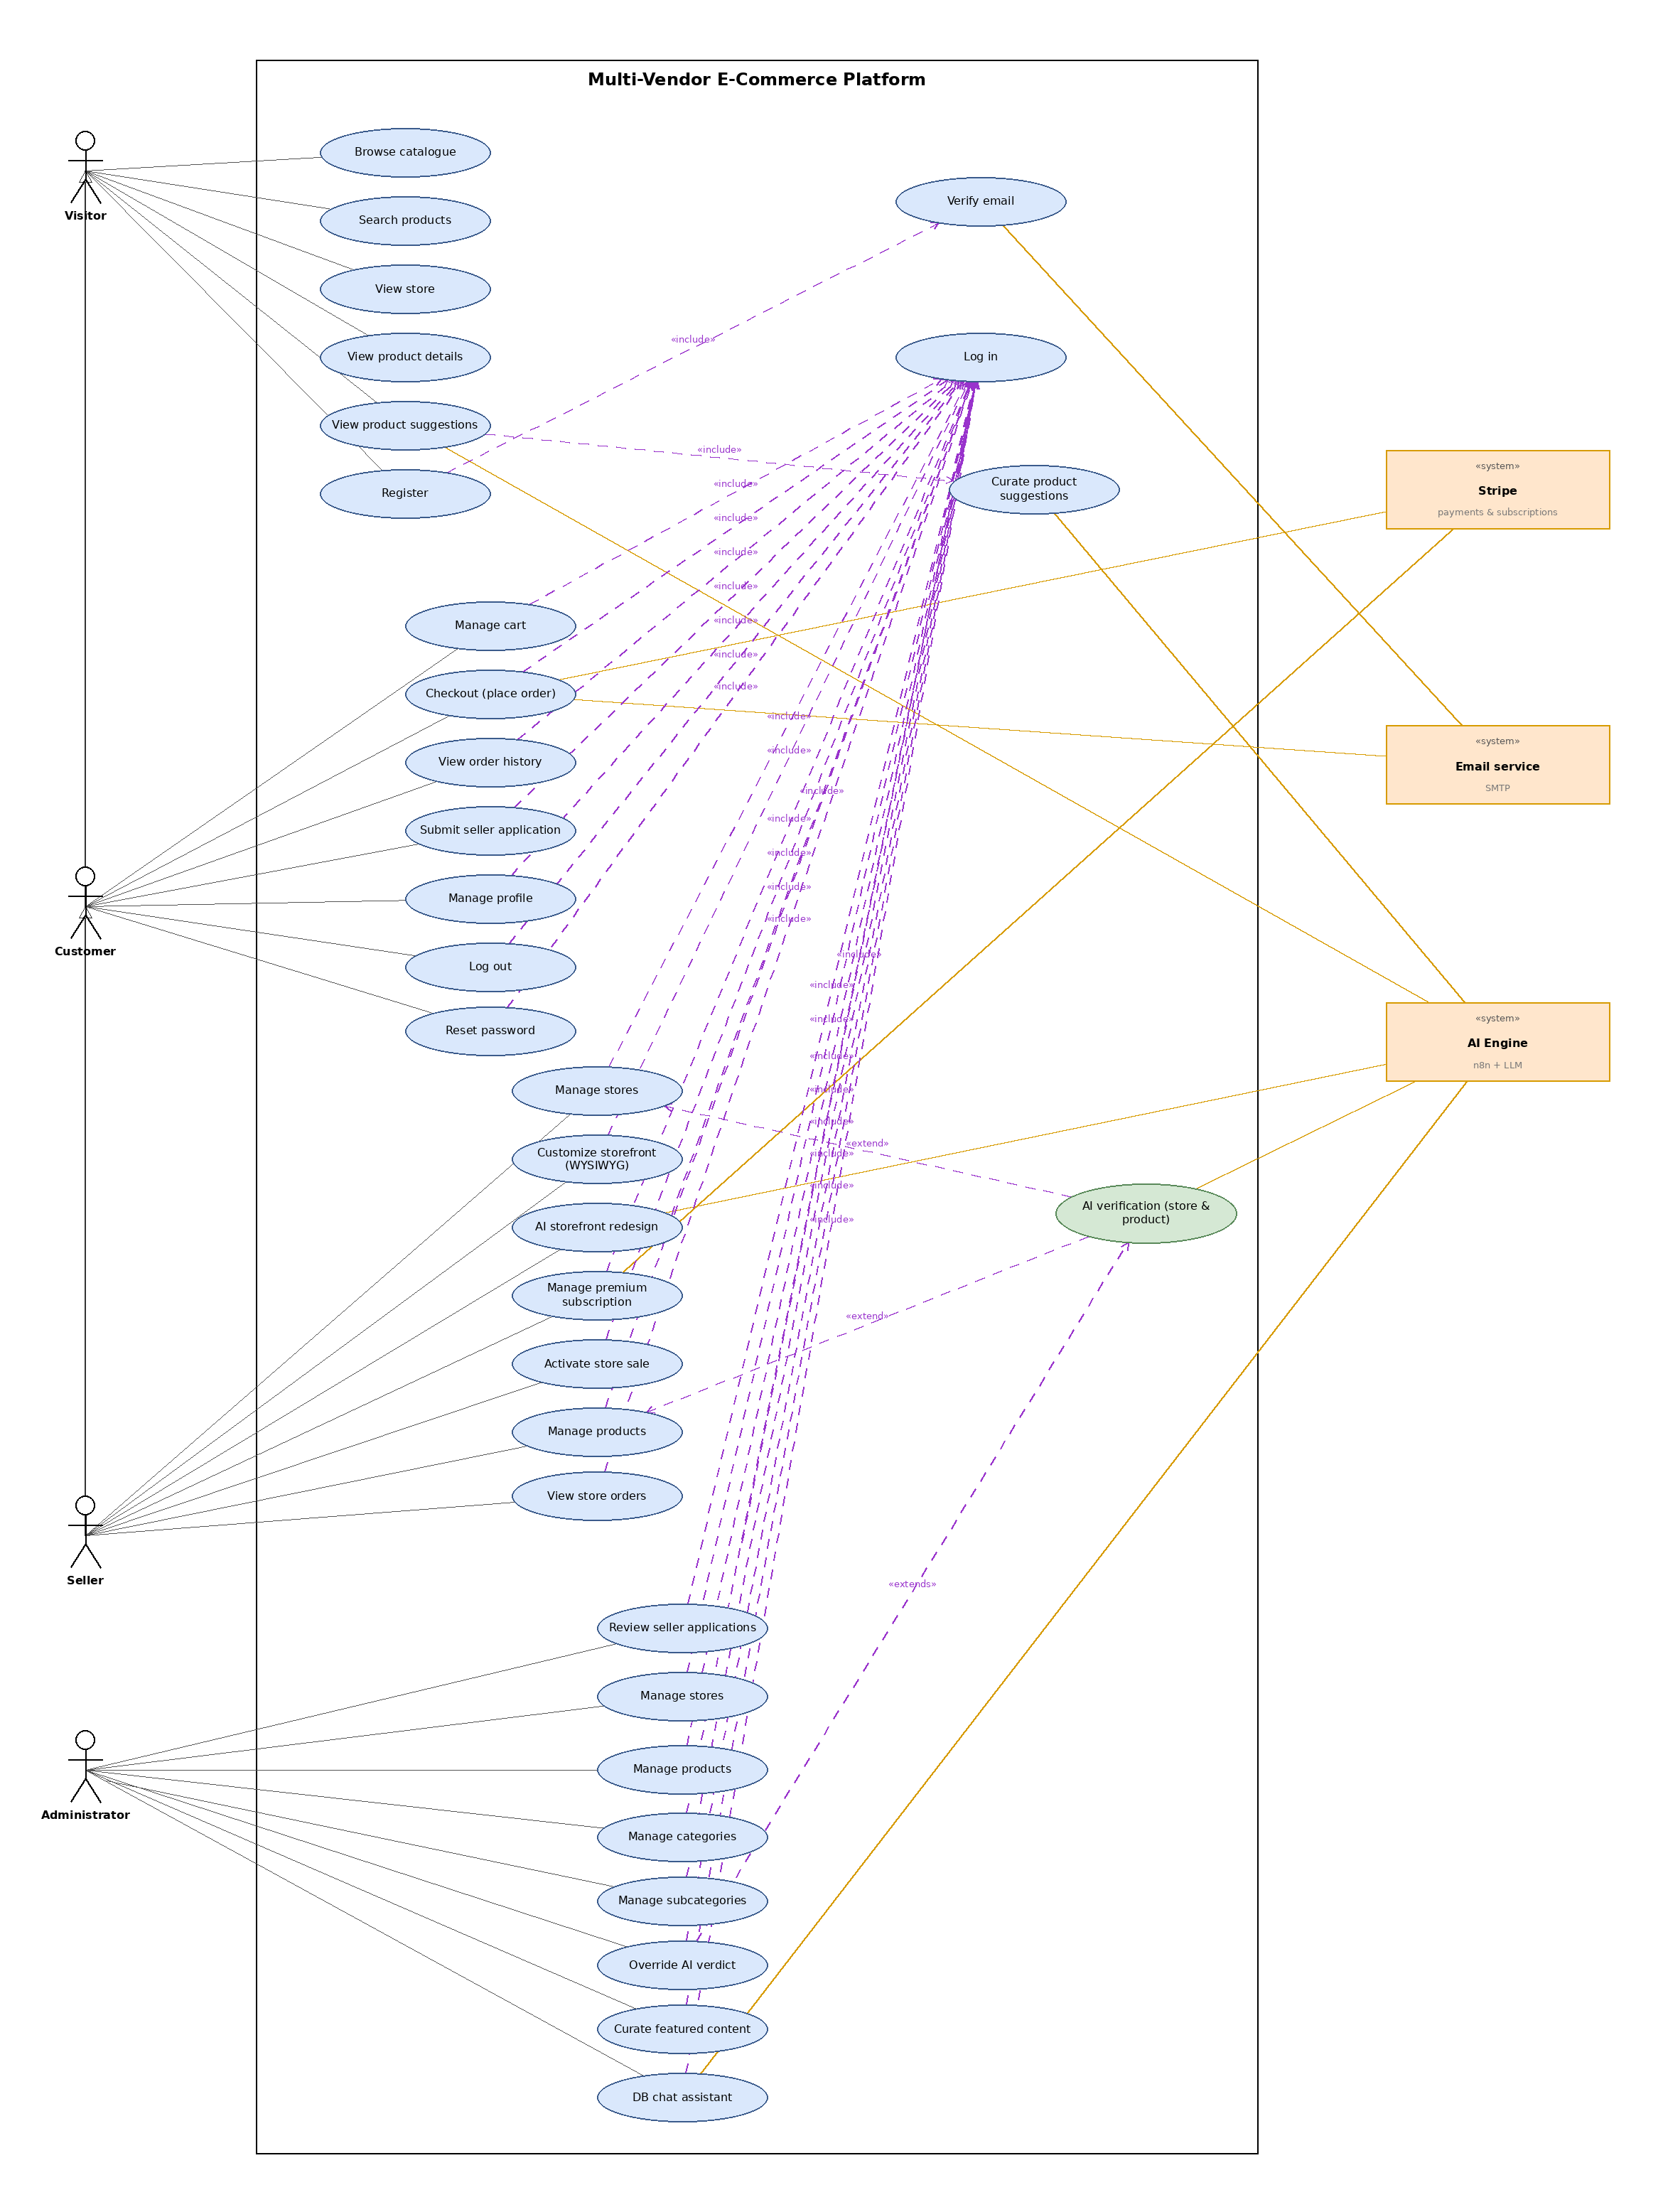
\includegraphics[height=0.86\textheight,keepaspectratio]{img/uc-global.png}
  \caption{Global use-case diagram}
  \label{fig:uc-global}
\end{figure}

\section{Class Diagram}

Figure~\ref{fig:class} presents the static domain model. A single
\texttt{User} entity carries the customer, seller and administrator
roles, together with the premium-subscription and Stripe billing
attributes (\texttt{isPremium}, \texttt{premiumExpiresAt} and the Stripe
customer and subscription identifiers); a Seller owns one or more
\texttt{Store} entities, each holding \texttt{Product} entities that are
organised by \texttt{Category} and \texttt{Tag}; orders are modelled by an
\texttt{Order} aggregate and its \texttt{OrderItem} lines, allowing a
single checkout to span several stores.

\begin{figure}[H]
  \centering
  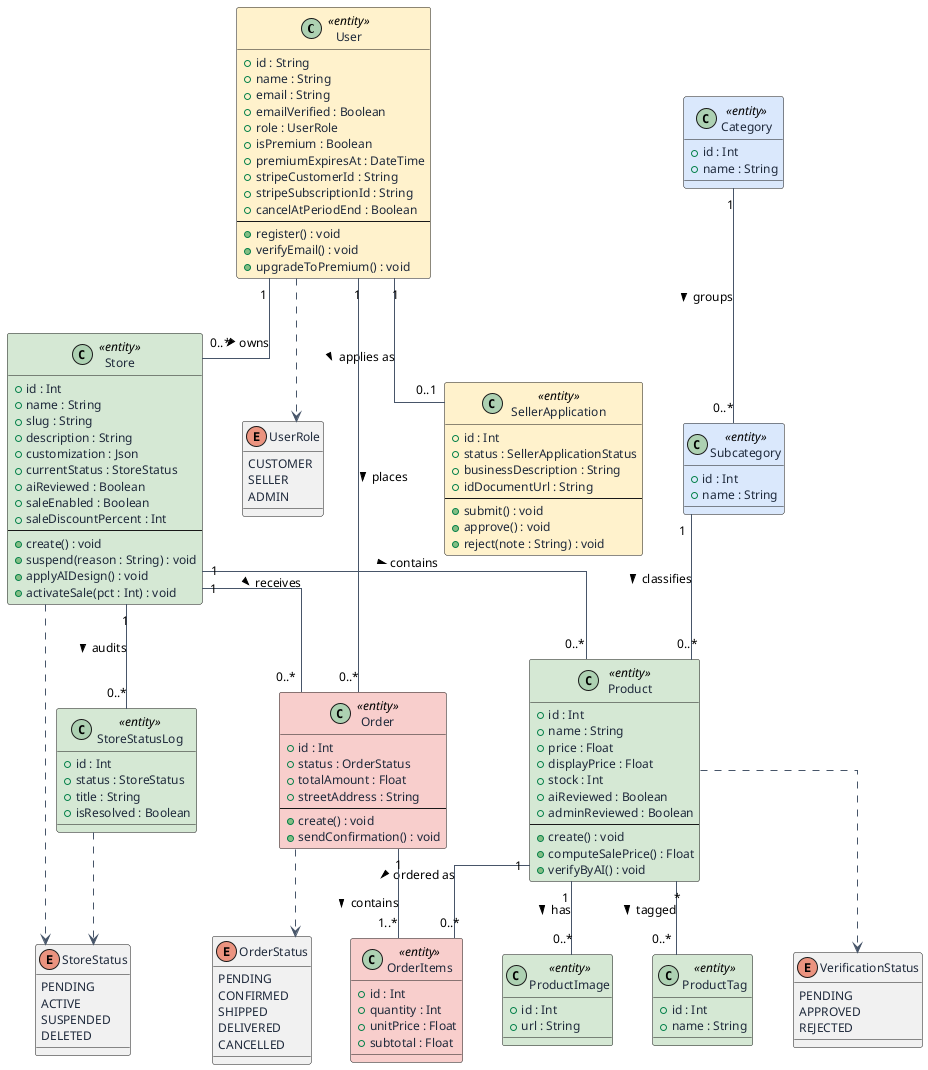
\includegraphics[width=\columnwidth,keepaspectratio]{img/class-diagram.png}
  \caption{Class diagram of the platform domain model}
  \label{fig:class}
\end{figure}

\section{Project Management with Scrum}

\subsection{Scrum Team}

The Scrum accountabilities were distributed as follows:

\begin{itemize}[leftmargin=*,itemsep=2pt]
  \item \textbf{Product Owner:} Mr.\ Mohammed Aziz Chibani (NeuralBey),
        who owned the product vision and prioritised the backlog.
  \item \textbf{Scrum Master and Development Team:} Nadim Jebali (the
        student), responsible for applying the framework and for the
        entire technical realisation.
\end{itemize}

\subsection{MoSCoW Priority Legend}

Each user story carries a \textbf{MoSCoW} priority and a
\textbf{complexity} estimate, defined in Table~\ref{tab:moscow}.

\begin{table}[H]
  \centering
  \caption{MoSCoW priority and complexity legend}
  \label{tab:moscow}
  \begin{tabularx}{\textwidth}{lllX}
    \toprule
    \multicolumn{4}{c}{\textbf{MoSCoW Priority}} \\
    \midrule
    \cellcolor{moscowMust}\textbf{Must}     & \textit{Must have}   & & Essential feature, required for the MVP. \\
    \cellcolor{moscowShould}\textbf{Should} & \textit{Should have} & & Important but not blocking. \\
    \cellcolor{moscowCould}\textbf{Could}   & \textit{Could have}  & & Desirable, included if time permits. \\
    \cellcolor{moscowWont}\textbf{Won't}    & \textit{Won't have}  & & Out of scope for this version. \\
    \midrule
    \multicolumn{4}{c}{\textbf{Complexity}} \\
    \midrule
    \cellcolor{complexLow}\textbf{1}   & Simple       & & Straightforward implementation, minimal effort. \\
    \cellcolor{complexMed}\textbf{2}   & Moderate     & & Average complexity, moderate effort. \\
    \cellcolor{complexHigh}\textbf{3}  & Complex      & & Significant effort, elaborate logic. \\
    \cellcolor{complexVHigh}\textbf{5} & Very complex & & High effort, advanced technical challenge. \\
    \bottomrule
  \end{tabularx}
\end{table}

\subsection{Product Backlog}

Table~\ref{tab:backlog} presents the product backlog as user stories
following the template \textit{``As a \textless role\textgreater, I want
\textless action\textgreater\ so that \textless benefit\textgreater''}.
The columns \textbf{P} and \textbf{Cx} indicate the MoSCoW priority and
the estimated complexity.

\setlength{\extrarowheight}{3pt}
\begin{longtable}{|>{\centering\arraybackslash\small}p{2.2cm}|>{\centering\arraybackslash\small}p{0.9cm}|>{\small}p{7.4cm}|>{\centering\arraybackslash\small}p{1.3cm}|>{\centering\arraybackslash\small}p{0.6cm}|}
  \caption{Product backlog --- user stories with MoSCoW priority and complexity}
  \label{tab:backlog}\\
  \hline
  \rowcolor{tableHeader}
  \textcolor{white}{\textbf{Feature}} & \textcolor{white}{\textbf{ID}} &
  \textcolor{white}{\textbf{User Story}} & \textcolor{white}{\textbf{P}} &
  \textcolor{white}{\textbf{Cx}} \\ \hline
  \endfirsthead
  \hline
  \rowcolor{tableHeader}
  \textcolor{white}{\textbf{Feature}} & \textcolor{white}{\textbf{ID}} &
  \textcolor{white}{\textbf{User Story}} & \textcolor{white}{\textbf{P}} &
  \textcolor{white}{\textbf{Cx}} \\ \hline
  \endhead
  \hline \multicolumn{5}{r|}{\small\textit{Continued on next page}}\\
  \endfoot
  \hline
  \endlastfoot

  \cellcolor{featAuth}\makecell[c]{\textbf{F1}\\\small Authentication}
  & US01 & As a visitor, I want to create an account with my email so that I can access the platform. & \cellcolor{moscowMust}\textbf{Must} & \cellcolor{complexMed}\textbf{2} \\\hline
  \cellcolor{featAuth}~ & US02 & As a visitor, I want a verification email so that I can activate my account securely. & \cellcolor{moscowMust}\textbf{Must} & \cellcolor{complexMed}\textbf{2} \\\hline
  \cellcolor{featAuth}~ & US03 & As a user, I want to sign in with my credentials so that I can access my dashboard. & \cellcolor{moscowMust}\textbf{Must} & \cellcolor{complexLow}\textbf{1} \\\hline
  \cellcolor{featAuth}~ & US04 & As a user, I want to sign out so that I can protect my account on a shared device. & \cellcolor{moscowMust}\textbf{Must} & \cellcolor{complexLow}\textbf{1} \\\hline
  \cellcolor{featAuth}~ & US37 & As a user, I want to reset my password by email when I forget it so that I can regain access to my account. & \cellcolor{moscowShould}\textbf{Should} & \cellcolor{complexMed}\textbf{2} \\\hline

  \cellcolor{featStore}\makecell[c]{\textbf{F2}\\\small Store\\Management}
  & US05 & As a seller, I want to create a store with a name, description and logo so that customers can recognise my brand. & \cellcolor{moscowMust}\textbf{Must} & \cellcolor{complexMed}\textbf{2} \\\hline
  \cellcolor{featStore}~ & US06 & As a seller, I want my store URL to use a readable slug so that it is easy to share. & \cellcolor{moscowMust}\textbf{Must} & \cellcolor{complexMed}\textbf{2} \\\hline
  \cellcolor{featStore}~ & US07 & As a seller, I want to customise my storefront across seven sections through a WYSIWYG editor so that I can style my store live. & \cellcolor{moscowShould}\textbf{Should} & \cellcolor{complexVHigh}\textbf{5} \\\hline
  \cellcolor{featStore}~ & US08 & As a seller, I want to apply a preset so that I can get a professional look quickly. & \cellcolor{moscowShould}\textbf{Should} & \cellcolor{complexMed}\textbf{2} \\\hline
  \cellcolor{featStore}~ & US09 & As a premium seller, I want to operate multiple stores so that I can segment my offerings. & \cellcolor{moscowShould}\textbf{Should} & \cellcolor{complexMed}\textbf{2} \\\hline
  \cellcolor{featStore}~ & US34 & As a seller, I want a store-wide percentage sale so that all my products show discounted prices and a badge automatically. & \cellcolor{moscowShould}\textbf{Should} & \cellcolor{complexMed}\textbf{2} \\\hline

  \cellcolor{featProduct}\makecell[c]{\textbf{F3}\\\small Product\\Management}
  & US10 & As a seller, I want to create, edit and delete products so that I can keep my catalogue up to date. & \cellcolor{moscowMust}\textbf{Must} & \cellcolor{complexMed}\textbf{2} \\\hline
  \cellcolor{featProduct}~ & US11 & As a seller, I want to upload multiple product images so that customers can see my products clearly. & \cellcolor{moscowMust}\textbf{Must} & \cellcolor{complexMed}\textbf{2} \\\hline
  \cellcolor{featProduct}~ & US12 & As a seller, I want to assign tags to products so that the recommendation engine can surface them. & \cellcolor{moscowShould}\textbf{Should} & \cellcolor{complexLow}\textbf{1} \\\hline
  \cellcolor{featProduct}~ & US13 & As a customer, I want to browse products by category so that I can discover relevant items. & \cellcolor{moscowMust}\textbf{Must} & \cellcolor{complexLow}\textbf{1} \\\hline

  \cellcolor{featOrder}\makecell[c]{\textbf{F4}\\\small Order\\System}
  & US14 & As a customer, I want to add products to a cart so that I can purchase multiple items at once. & \cellcolor{moscowMust}\textbf{Must} & \cellcolor{complexMed}\textbf{2} \\\hline
  \cellcolor{featOrder}~ & US15 & As a customer, I want to check out across multiple stores in a single order so that I avoid separate transactions. & \cellcolor{moscowMust}\textbf{Must} & \cellcolor{complexHigh}\textbf{3} \\\hline
  \cellcolor{featOrder}~ & US16 & As a customer, I want a confirmation email after ordering so that I have a record of my purchase. & \cellcolor{moscowMust}\textbf{Must} & \cellcolor{complexLow}\textbf{1} \\\hline
  \cellcolor{featOrder}~ & US17 & As a seller, I want to view orders containing my products so that I can fulfil them. & \cellcolor{moscowMust}\textbf{Must} & \cellcolor{complexMed}\textbf{2} \\\hline
  \cellcolor{featOrder}~ & US36 & As a customer, I want to pay securely for my order online so that my purchase is confirmed instantly. & \cellcolor{moscowMust}\textbf{Must} & \cellcolor{complexHigh}\textbf{3} \\\hline

  \cellcolor{featAdmin}\makecell[c]{\textbf{F5}\\\small Administration}
  & US18 & As an admin, I want to review seller applications so that I can approve legitimate merchants. & \cellcolor{moscowMust}\textbf{Must} & \cellcolor{complexMed}\textbf{2} \\\hline
  \cellcolor{featAdmin}~ & US19 & As an admin, I want to suspend or delete any store so that I can enforce marketplace rules. & \cellcolor{moscowMust}\textbf{Must} & \cellcolor{complexMed}\textbf{2} \\\hline
  \cellcolor{featAdmin}~ & US20 & As an admin, I want to curate featured stores and products so that the landing page promotes quality. & \cellcolor{moscowShould}\textbf{Should} & \cellcolor{complexLow}\textbf{1} \\\hline
  \cellcolor{featAdmin}~ & US21 & As an admin, I want to manage categories so that the catalogue stays organised. & \cellcolor{moscowMust}\textbf{Must} & \cellcolor{complexLow}\textbf{1} \\\hline

  \cellcolor{featAI}\makecell[c]{\textbf{F6}\\\small AI\\Verification}
  & US22 & As the system, I want to verify every new store and product via an LLM so that low-quality content is flagged automatically. & \cellcolor{moscowShould}\textbf{Should} & \cellcolor{complexHigh}\textbf{3} \\\hline
  \cellcolor{featAI}~ & US23 & As an admin, I want to override any AI verdict so that I remain the final authority. & \cellcolor{moscowMust}\textbf{Must} & \cellcolor{complexLow}\textbf{1} \\\hline
  \cellcolor{featAI}~ & US24 & As a customer, I want an AI-verified badge on trusted products so that I can shop with confidence. & \cellcolor{moscowShould}\textbf{Should} & \cellcolor{complexLow}\textbf{1} \\\hline
  \cellcolor{featAI}~ & US35 & As a seller, I want to regenerate my storefront from a natural-language prompt so that I get a professional design without manual work. & \cellcolor{moscowCould}\textbf{Could} & \cellcolor{complexHigh}\textbf{3} \\\hline

  \cellcolor{featPremium}\makecell[c]{\textbf{F7}\\\small Premium\\Tier}
  & US25 & As a seller, I want to subscribe to a premium plan so that I can unlock advanced features. & \cellcolor{moscowShould}\textbf{Should} & \cellcolor{complexHigh}\textbf{3} \\\hline
  \cellcolor{featPremium}~ & US26 & As a premium seller, I want all customisation controls so that I can fully personalise my store. & \cellcolor{moscowShould}\textbf{Should} & \cellcolor{complexHigh}\textbf{3} \\\hline
  \cellcolor{featPremium}~ & US27 & As the system, I want to preserve premium customisation after expiry so that the store keeps its design. & \cellcolor{moscowCould}\textbf{Could} & \cellcolor{complexMed}\textbf{2} \\\hline

  \cellcolor{featCICD}\makecell[c]{\textbf{F8}\\\small CI/CD \&\\Deployment}
  & US28 & As a developer, I want every service in a Docker container so that environments are identical. & \cellcolor{moscowMust}\textbf{Must} & \cellcolor{complexMed}\textbf{2} \\\hline
  \cellcolor{featCICD}~ & US29 & As a developer, I want images built and pushed automatically on every push to main so that deployments are current. & \cellcolor{moscowMust}\textbf{Must} & \cellcolor{complexMed}\textbf{2} \\\hline
  \cellcolor{featCICD}~ & US30 & As a developer, I want the droplet provisioned via Terraform so that infrastructure is reproducible. & \cellcolor{moscowShould}\textbf{Should} & \cellcolor{complexHigh}\textbf{3} \\\hline
  \cellcolor{featCICD}~ & US31 & As a developer, I want deployment over SSH on every push to main so that updates reach production automatically. & \cellcolor{moscowMust}\textbf{Must} & \cellcolor{complexHigh}\textbf{3} \\\hline
  \cellcolor{featCICD}~ & US32 & As a developer, I want secrets managed through CI secrets so that no credentials live in the repository. & \cellcolor{moscowMust}\textbf{Must} & \cellcolor{complexLow}\textbf{1} \\\hline
  \cellcolor{featCICD}~ & US33 & As a developer, I want DNS records updated automatically to the new droplet IP so that the application is always reachable. & \cellcolor{moscowShould}\textbf{Should} & \cellcolor{complexMed}\textbf{2} \\\hline

  \cellcolor{featAccount}\makecell[c]{\textbf{F9}\\\small Account\\Management}
  & US38 & As a user, I want to view and edit my profile and change my password so that I can keep my account details current and secure. & \cellcolor{moscowMust}\textbf{Must} & \cellcolor{complexMed}\textbf{2} \\\hline
  \cellcolor{featAccount}~ & US39 & As a customer, I want to consult my purchase history so that I can review my past orders. & \cellcolor{moscowShould}\textbf{Should} & \cellcolor{complexLow}\textbf{1} \\\hline

  \cellcolor{featTheme}\makecell[c]{\textbf{F10}\\\small Appearance\\\& Theming}
  & US40 & As a user, I want to switch between a light and a dimmed dark theme, or follow my system preference, so that I can browse comfortably in low light. & \cellcolor{moscowCould}\textbf{Could} & \cellcolor{complexMed}\textbf{2} \\\hline

\end{longtable}

\subsection{Analysis Summary}

The product backlog comprises \textbf{40 user stories} across
\textbf{10 features}. The bulk are \textit{Must} or \textit{Should}
priorities forming the marketplace core, while a few advanced
capabilities (AI redesign, premium-customisation preservation) are
\textit{Could} items scheduled only once the essentials are delivered.
Complexity estimates concentrate effort on the storefront editor, the
multi-store checkout, the AI verification pipeline and the deployment
automation.

\subsection{Sprint Planning per Release}

The backlog was organised into \textbf{two releases of two sprints
each}. The first release delivers the social and transactional
foundations; the second adds intelligence, monetisation and the
deployment pipeline. Table~\ref{tab:sprints} maps each sprint to its
goal and user stories.

\begin{table}[H]
  \centering
  \caption{Sprint planning across the two releases}
  \label{tab:sprints}
  \begin{tabularx}{\textwidth}{|l|l|X|>{\centering\arraybackslash}p{2.9cm}|}
    \hline
    \rowcolor{tableHeader}
    \textcolor{white}{\textbf{Release}} & \textcolor{white}{\textbf{Sprint}} &
    \textcolor{white}{\textbf{Goal}} & \textcolor{white}{\textbf{User stories}} \\
    \hline
    \multirow{2}{*}{\textbf{Release 1}}
      & Sprint 1 & Authentication and seller onboarding & US01--US04, US18, US37 \\
    \cline{2-4}
      & Sprint 2 & Store and product management & US05--US13, US34 \\
    \hline
    \multirow{2}{*}{\textbf{Release 2}}
      & Sprint 3 & Orders, payment, account and administration & US14--US17, US19--US21, US36, US38, US39 \\
    \cline{2-4}
      & Sprint 4 & AI verification, premium tier, theming and DevOps & US22--US33, US35, US40 \\
    \hline
  \end{tabularx}
\end{table}

\section{Gantt Diagram}

Figure~\ref{fig:gantt} presents the project schedule over the
internship: an inception phase, the four sprints grouped into two
releases with their delivery milestones, a tests-and-deployment phase,
and a report-writing activity running in parallel throughout.

\begin{figure}[H]
  \centering
  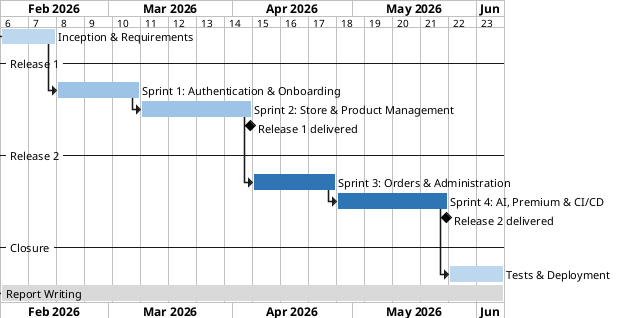
\includegraphics[width=\columnwidth,keepaspectratio]{img/gantt.png}
  \caption{Project Gantt chart (two releases, four sprints)}
  \label{fig:gantt}
\end{figure}

\section{Architecture and Technical Choices}

\subsection{Logical Architecture}

The platform follows a classic \textbf{three-tier architecture} that
separates the user interface (presentation), the business logic
(application) and the persistent data (data) into independent layers,
with an \textbf{n8n} automation layer orbiting the backend to host the
AI workflows. End users reach the platform over HTTPS; a reverse proxy
serves the React bundle and forwards \texttt{/api/*} requests to the
NestJS API, which persists state to MariaDB through Prisma and exchanges
webhooks with n8n. Figure~\ref{fig:arch-logic} shows the topology.

\begin{figure}[H]
  \centering
  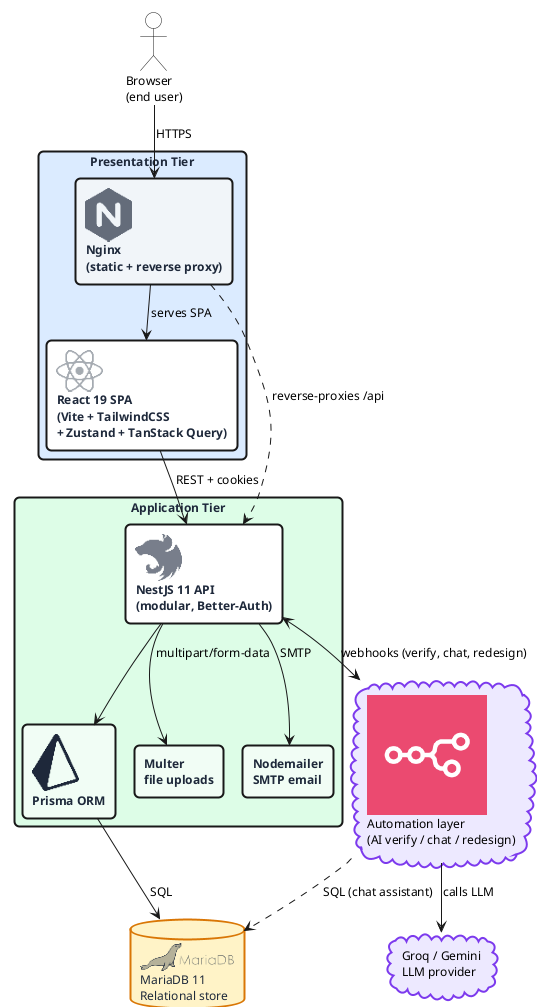
\includegraphics[width=\columnwidth,height=0.62\textheight,keepaspectratio]{img/arch-3tier-v2.png}
  \caption{Logical architecture (three tiers and the n8n automation layer)}
  \label{fig:arch-logic}
\end{figure}

\subsection{Physical Architecture}

In production, every component runs as a \textbf{Docker} container
orchestrated by Docker Compose on a single DigitalOcean droplet. A
\textbf{Caddy} reverse proxy terminates TLS with automatically renewed
Let's Encrypt certificates and routes traffic to the frontend, backend
and n8n containers over an internal bridge network; uploads and the n8n
state persist on Docker volumes. Figure~\ref{fig:arch-phys} details the
container topology.

\begin{figure}[H]
  \centering
  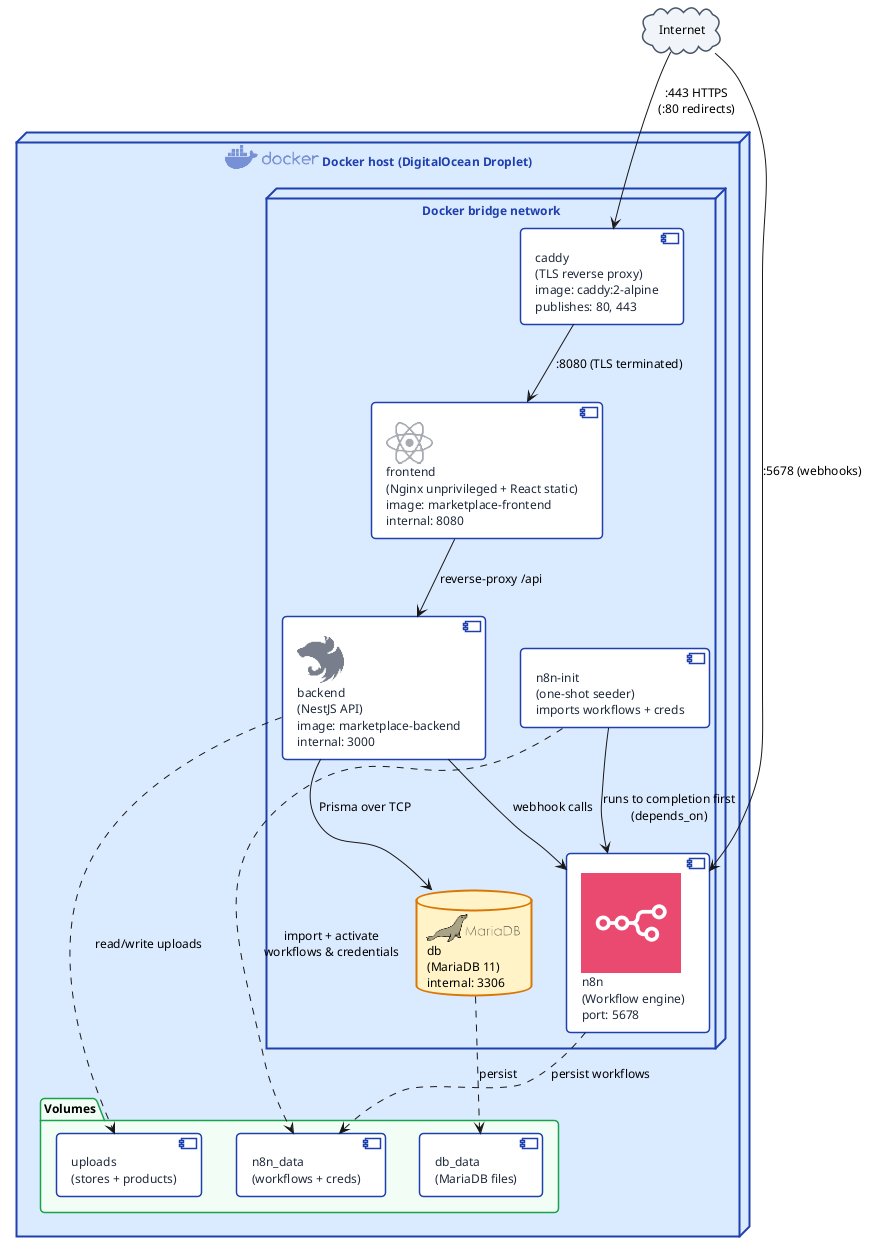
\includegraphics[width=\columnwidth,height=0.85\textheight,keepaspectratio]{img/arch-docker-v2.png}
  \caption{Physical architecture (Docker Compose services)}
  \label{fig:arch-phys}
\end{figure}

\subsection{Artificial-Intelligence Models}

The intelligent features are powered by hosted large-language models,
orchestrated through n8n so that providers can be swapped without
touching the backend. Table~\ref{tab:aimodels} lists the model used by
each service.

\begin{table}[H]
  \centering
  \caption{AI models used per service}
  \label{tab:aimodels}
  \begin{tabularx}{\textwidth}{|l|X|}
    \hline
    \rowcolor{tableHeader}
    \textcolor{white}{\textbf{Service}} & \textcolor{white}{\textbf{Model / provider}} \\
    \hline
    Store and product verification & Multimodal LLM (Google Gemini~\cite{gemini}) screening images and listing text \\ \hline
    AI storefront redesign         & Groq~\cite{groq} \texttt{llama-3.3-70b-versatile} generating the storefront customisation \\ \hline
    Database chat assistant        & Hosted LLM translating natural-language questions into safe database queries \\ \hline
  \end{tabularx}
\end{table}

\subsection{Tools, Frameworks and Languages}

The system is implemented in \textbf{TypeScript} end to end.
Table~\ref{tab:tools} lists the tools used throughout the project ---
covering source control, project tracking, development,
containerisation, infrastructure provisioning, workflow automation and
API testing --- while Table~\ref{tab:frameworks} summarises the main
frameworks and libraries.

\begin{table}[H]
  \centering
  \caption{Tools used throughout the project}
  \label{tab:tools}
  \begin{tabular}{|>{\centering\arraybackslash}m{1.4cm}|l|m{8.2cm}|}
    \hline
    \rowcolor{tableHeader}
    \textcolor{white}{\textbf{Logo}} & \textcolor{white}{\textbf{Tool}} & \textcolor{white}{\textbf{Role}} \\
    \hline
    
\includegraphics[height=0.8cm]{img/github.png}    & GitHub~\cite{github}       & Version control, pull-request review and CI/CD via GitHub Actions. \\ \hline
    
\includegraphics[height=0.8cm]{img/notion.png}    & Notion~\cite{notion}       & Backlog management, task board and record of user stories. \\ \hline
    
\includegraphics[height=0.8cm]{img/vscode.png}    & VS Code~\cite{vscode}      & Primary IDE, extended for TypeScript, Prisma, ESLint and Git. \\ \hline
    
\includegraphics[height=0.8cm]{img/docker.png}    & Docker~\cite{docker}       & Containerisation of all services for dev/prod parity. \\ \hline
    
\includegraphics[height=0.8cm]{img/terraform.png} & Terraform~\cite{terraform} & Infrastructure-as-code provisioning of the DigitalOcean resources. \\ \hline
    
\includegraphics[height=0.8cm]{img/n8n.png}       & n8n~\cite{n8n}             & Visual workflow automation orchestrating the AI features. \\ \hline
    
\includegraphics[height=0.8cm]{img/postman.png}   & Postman~\cite{postman}     & Manual testing and documentation of the REST endpoints. \\ \hline
    
\includegraphics[height=0.8cm]{img/pnpm.png}      & pnpm~\cite{pnpm}           & Fast, disk-efficient package manager for the monorepo. \\ \hline
  \end{tabular}
\end{table}

\begin{table}[H]
  \centering
  \caption{Frameworks and languages}
  \label{tab:frameworks}
  \begin{tabularx}{\textwidth}{|l|X|}
    \hline
    \rowcolor{tableHeader}
    \textcolor{white}{\textbf{Technology}} & \textcolor{white}{\textbf{Role}} \\
    \hline
    TypeScript~\cite{typescript}  & Statically-typed language used across the frontend and the backend. \\ \hline
    React~\cite{react}            & Single-page application library for the customer, seller and admin interfaces. \\ \hline
    NestJS~\cite{nestjs}          & Modular Node.js framework structuring the backend into feature modules. \\ \hline
    Prisma~\cite{prisma}          & ORM and migration tool over MariaDB. \\ \hline
    Better-Auth~\cite{betterauth} & Authentication library handling sessions and email verification. \\ \hline
    Docker        & Container runtime packaging every service. \\ \hline
    Terraform     & Declarative provisioning of the cloud infrastructure. \\ \hline
    n8n           & Workflow engine hosting the AI orchestration. \\ \hline
  \end{tabularx}
\end{table}

\subsection{Database}

The platform stores its data in a \textbf{MariaDB}~\cite{mariadb}
relational database accessed through the \textbf{Prisma} ORM, which provides a type-safe
client and versioned migrations. The database schema follows directly
from the domain model: the entities and associations of the class
diagram presented earlier (Figure~\ref{fig:class}) map onto the database
tables --- users and their roles, stores and their customisation,
products with categories and tags, and orders with their line items ---
with Prisma generating and versioning the corresponding migrations.

\begin{figure}[H]
  \centering
  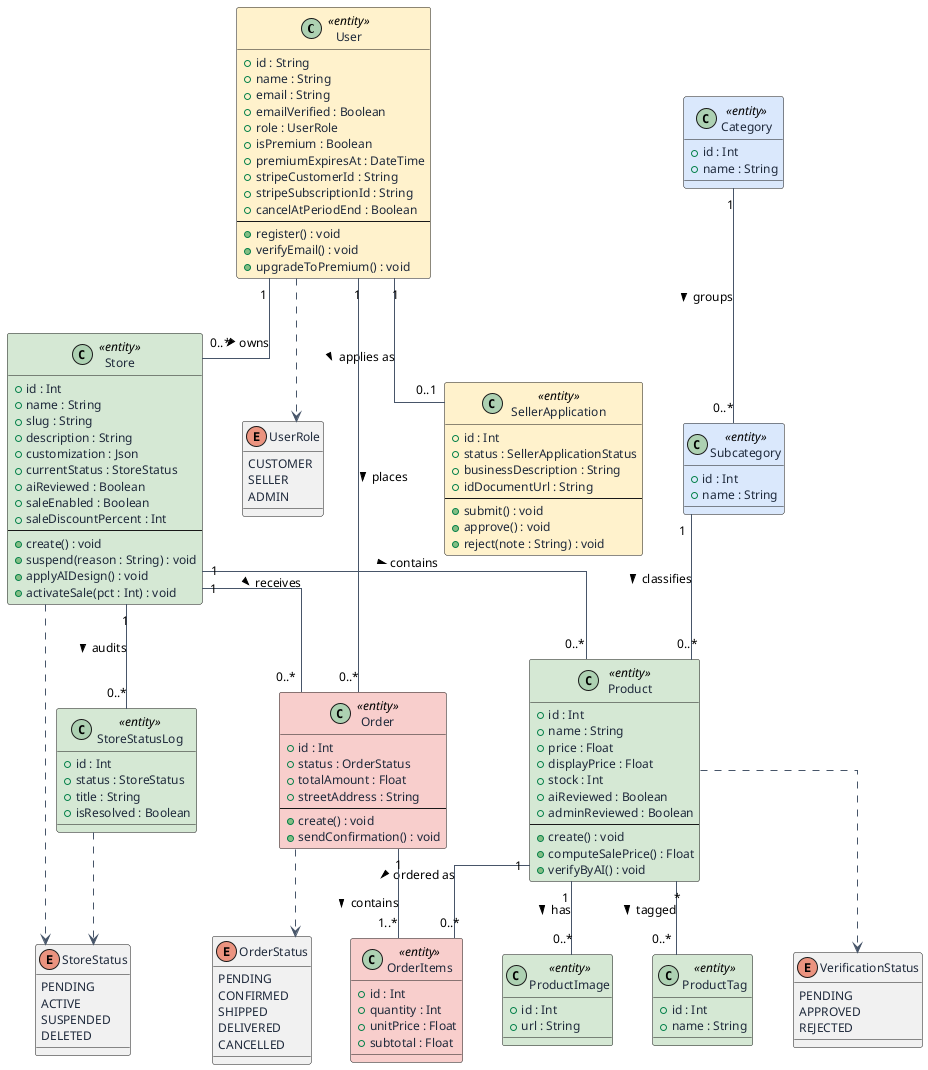
\includegraphics[width=\columnwidth,keepaspectratio]{img/class-diagram.png}
  \caption{Class diagram underpinning the database schema}
  \label{fig:db-class}
\end{figure}

\section*{Conclusion}

This chapter formalised the requirements of the platform. The three
actors were identified, the functional requirements grouped into seven
domains and the non-functional requirements stated, then illustrated
with the global use-case diagram and the class diagram. The Scrum
management of the project was presented --- the team, the MoSCoW-prioritised
product backlog of 40 user stories across 10 features, and the planning
of four sprints over two releases --- together with the schedule and the
architecture and technical choices that frame the realisation. The
following chapters describe the development of the two releases.
